\documentclass{report}

\usepackage{graphicx}
\usepackage{float}
\usepackage{hyperref}
\usepackage{listings}
\usepackage{hyperref}

\begin{document}

\title{\huge{\textbf{BosHBus: Transporte de trabalhadores}} \\ CAL 2019/2020 \\ MIEIC FEUP}
  \author{João de Jesus Costa \\ \texttt{up201806560} \\ \texttt{joao.jcosta@fe.up.pt} \and
          João Lucas Silva Martins \\ \texttt{up201806436} \\ \texttt{up201806436@fe.up.pt} \and
          Tiago Duarte da Silva \\ \texttt{up201806516} \\ \texttt{up201806516@fe.up.pt}
          }
  \date{\today{}}

  \begin{figure}[b]
    \centering
      
\includegraphics[width=0.6\textwidth]{img/feup_logo.png}
  \end{figure}
\maketitle{}

\tableofcontents{}
\newpage

\chapter{Descrição do tema}
  \section{Descrição sucinta do problema}
    Uma empresa de transportes especializa-se em transportes de trabalhadores no
    percurso \textit{casa-trabalho} (e vice-versa) de forma eficiente. Para isso,
    dispõe de veículos que precisam de fazer o percurso de uma garagem até à empresa
    cliente, passando por diversos pontos de encontro onde estarão os
    trabalhadores a transportar. No final do dia de trabalho, o transporte fará
    o percurso inverso.\\
    Podem existir diversos pontos de encontro de modo a que os trabalhadores
    consigam facilmente chegar desde suas casas ao seu designado ponto.\\
    Inicialmente, a empresa de transporte possui apenas um veículo e fornece os
    seus serviços a apenas uma outra empresa. No entanto, o número de veículos
    e empresas clientes poderá vir a aumentar ao longo do tempo, acompanhando a
    expansão da empresa.\\
    \newline
    Este problema pode ser dividido em quatro partes.
  
  \section{Escolha de pontos de encontro e seu número}
    É necessário definir uma distância máxima a que a casa de um trabalhador
    pode estar em relação ao ponto de encontro mais próximo. Esta distância
    tem de ser pequena o suficiente para que qualquer trabalhador se consiga
    deslocar a pé até esse ponto de encontro (e posteriormente até casa) em
    pouco tempo.\\
    Com base nessa distância, é possível definir a quantidade mínima de pontos
    e as suas posições para recolher todos os trabalhadores.\\
    \newline
    Com isto, podemos ver que o grafo terá quatro tipos de nós: o nó de origem,
    os nós de destino, os nós marcados como ponto de encontro e os restantes
    nós (sem nenhuma nomenclatura especial).

  \section{Cálculo da rota mais curta}
    Depois de todos os pontos de encontro serem conhecidos, é necessário
    calcular a melhor rota para o transporte seguir.\\
    A melhor rota é definida como: a rota mais curta que parte da garagem do
    autocarro e termina na empresa cliente, passando por todos os pontos de
    encontro pelo menos uma vez.\\
    Esta rota será seguida pelo autocarro em ambos os sentidos, ou seja, da garagem
    à empresa cliente e da empresa cliente à garagem.\\
    É necessário ter em atenção que obras podem tornar certas vias inacessíveis.
    \newline
    Nesta fase do problema, assumimos que o autocarro tem capacidade para
    transportar todos os trabalhadores na sua rota.

  \section{Determinação de rotas para vários autocarros (um só destino)}
    É possível que um autocarro não tenha capacidade para transportar todos os
    trabalhadores de uma empresa cliente de uma só vez.\\
    Para isto, será necessário calcular o número mínimo de veículos necessários
    para transportar todos os trabalhadores e a melhor rota para cada um desses
    veículos.\\
    \newline
    É de notar que, mesmo que um autocarro tenha capacidade para fazer uma rota
    completa sozinho, usar mais autocarros (caso estejam disponíveis) pode ser
    mais eficiente.

  \section{Determinação de rotas para vários autocarros (vários clientes)}
    Serão precisos vários autocarros para conseguir satisfazer os requerimentos
    de diversas empresas clientes ao mesmo tempo, visto que cada autocarro só
    tem uma empresa como destino.\\
    Este problema pode ser resolvido determinando uma rota para cada empresa
    de forma individual.

\newcommand{\arrou}[2] {$\hbox{#1} \rightarrow \hbox{#2}$}
\newcommand{\arrouline}[2] {$\hbox{\underline{#1}} \rightarrow \hbox{#2}$}

\chapter{Formalização do problema}
  \section{Definições base}
    \begin{itemize}
      \item $V$ é o conjunto de todos os nós do mapa. Cada nó representa uma
        intersecção entre duas ou mais vias.
      \item $i$ representa o índice de um nó no mapa.

      \item $E$ é o conjunto de todas as arestas do mapa. Cada aresta representa
        uma via no mapa.

      \item $G = (V, E)$ é um grafo dirigido, pesado e conexo, constituído por
        vértices e suas arestas. Cada aresta do grafo representa uma via e cada
        vértice representa uma intersecção entre duas ou mais vias.

      \item $C$ é a lista de empresas clientes e sua informação.
      \item $n$ representa o índice de uma empresa cliente na lista $clientes$.
    \end{itemize}

  \section{Dados de entrada}
    \begin{itemize}
    \item $d_{max}$ representa a distância máxima a que um ponto de encontro
      pode estar de um local de residência.
    \item $b_{num}$ representa o número de autocarros disponíveis.
    \item $b_{cap}$ representa capacidade (em número de pessoas) de cada
      autocarro disponível.

    \item Todas as interseções, $V_i$, de duas ou mais vias no mapa: $V_i \in V$
      é o nó de índice $i$ no grafo.
    \item O nó onde se localiza a garagem dos autocarros, $V_0 \in V$.

    \item Todas as vias, $i\rightarrow j$, no mapa: $i\rightarrow j \in E$
      representa uma aresta dirigida (pesada) desde o nó de índice $i$ até ao nó
      de índice $j$.
    \item O comprimento, $w_{ij}$, de todas as vias de comutação $i\rightarrow j$.
      $w_{ij}$ é o peso da aresta $i\rightarrow j$.

    \item A localização do local de trabalho dessa empresa, ou seja, o local
      onde os trabalhadores devem ser deixados, $D_{C_n}$, para cada empresa.
    \item A lista dos locais de residência, $H_{C_n}$, de cada trabalhador
      de cada empresa cliente.
    \end{itemize}
  \section{Dados de saída}
    \begin{itemize}
    \item A lista dos autocarros, $B$, a usar.
    \item $b$ é o índice de um autocarro na lista $B$.
    \item O comprimento, $L_{B_b}$, do caminho a ser percorrido por cada autocarro.
    \item A sequência ordenada, $P_{B_b} \in E$, de arestas a visitar por cada
      autocarro, terminando no ponto de destino.
    \item A lista de pontos de encontro, $M_{B_b} \in V$, que o autocarro vai visitar.
    \item A lista de passageiros, $T_{B_b}$, atribuídos a cada autocarro.

    \item A lista dos pontos de encontro, $M$, a usar (nós do grafo).
    \item $u$ representa o índice de um certo ponto de encontro na lista $M$.
    \item A lista dos trabalhadores, $W_{M_u}$, atribuídos ao ponto de encontro
      de índice $u$.
    \end{itemize}
    \newpage
  \section{Função objectivo}
    Minimizar o comprimento total do caminho percorrido:\\
    $min(\sum_{b \in B} L_{B_b})$
    \newline
    Minimizar o número total de autocarros usados:\\
    $min(|B|)$\\
    \newline
  \section{Restrições}
    Todos os pontos de encontro são atingidos:\\
    $\forall{m \in M}, \exists{p \in M_{B_b}} : m = p$\\
    \newline
    Todos os autocarros têm de chegar ao destino correto.\\
    Sendo $dest$ o último elemento da sequência ${B_b}_{m}$ e $D$ o destino da
    empresa cliente a que ${B_b}$ se refere, tem de se verificar:\\
    $\forall{b:{B_b} \in B} : dest = D$\\
    \newline
    Todos os trabalhadores têm de estar atribuídos a apenas um ponto de encontro.
    \newline
    Todos os trabalhadores têm de entrar no seu devido autocarro:\\
    $\forall{worker \in W_{M_y}}, worker \in T_{B_b}$

\chapter{Casos de utilização e funcionalidades}
  \section{Casos de utilização}
    Existem quatro casos possíveis de operação para a empresa \textbf{BosHBus},
    nos quais a empresa fornece os seus serviços a:
    \begin{itemize}
    \item um só cliente usando apenas um autocarro.
    \item um só cliente usando vários autocarros.
    \item a vários clientes usando apenas um autocarro para cada um deles.
    \item a vários clientes podendo usar um ou mais autocarros para cada um deles.
    \end{itemize}

  \section{Funcionalidades a implementar}
    Para a empresa \textbf{BosHBus} deverão ser implementadas as seguintes
    funcionalidades:
    \begin{itemize}
    \item Registo de um novo cliente (podem existir vários clientes registados).
    \item Remoção do registo de um cliente atual.
    \item Adicionar/remover autocarros da garagem (implica um possível atualização
      de todas as atuais rotas). É de notar que remover um autocarro pode, em certos
      casos, não ser possível dadas as necessidades dos atuais clientes.
    \end{itemize}
    \newpage
    Para as empresas clientes deverão ser implementadas as seguintes funcionalidades:
    \begin{itemize}
    \item Remover/Adicionar novos trabalhadores à sua empresa cliente.
    \item Atualizar a informação relativa aos trabalhadores da empresa.
    \item Atualizar o local de destino dos seus trabalhadores.
    \end{itemize}

\chapter{Formalização da Solução}
  \section{Prespetiva de solução}
    \subsection{Escolha de pontos de encontro}
      Uma solução alternativa à maximização do número de pontos de encontro
      também foi equacionada pelo grupo. Nesta estratégia, uma fila de 
      prioridade auxiliar com o máximo à cabeça é usada para armazenar os pontos
      de encontro. Os elementos são inseridos nesta fila de prioridade com base
      no número de trabalhadores que se encontram a uma distância aceitável desses
      (distância do trabalhador ao ponto $<= d_{max}$).
      \begin{itemize}
      \item $\forall{T \in H_{C_n}}$ de uma dada $C_n$, fazer uma pesquisa em
        profundidade pelas suas arestas adjacentes. A pesquisa num vértice pára
        quando a sua distância a $T$ ultrapassar $d_{max}$. Cada vértice alcançado
        que ainda não tenha sido visitado anteriormente deverá ser processado.
      \item Se o ponto de encontro referente ao vértice encontrado estiver na
        fila de prioridade então é lhe adicionado uma referência a $T$.\\
        Caso contrário, um novo ponto de encontro é adicionado à fila com uma
        referência ao trabalhador $T$.
      \item Quando todos os trabalhadores forem processados, a fila de prioridade
        deverá ser esvaziada, seguindo os seguintes passos:
        \begin{itemize}
        \item Extrair o ponto de encontro do topo da fila, adicionando-o à lista
          de resultados.
        \item Apagar todas as referências a trabalhadores que podem deslocar-se ao
          ponto retirado (no passo anterior).
        \item Atualizar a fila.
        \item Repetir até não haverem mais pontos de encontro na fila de prioridade.
        \end{itemize}
      \end{itemize}

      Uma estratégia descartada pelo grupo consistia em:
      \begin{itemize}
      \item Encontrar um grupo de trabalhadores com grande chance de poderem ter
        um ponto de encontro em comum, usando o primeiro método nesta secção.
      \item Usar o algoritmo de \textbf{dijsktra bidirecional} entre dois
        trabalhadores do grupo, escolhidos aleatoriamente.
      \item Obter o ponto de encontro dos dois algoritmos de \textbf{dijsktra} a
        correr em simultâneo.
      \item Executar os dois passos anteriores entre um outro trabalhador e o
        novo ponto obtido, até não haverem mais trabalhadores a processar.
      \end{itemize}
      Esta estratégia foi descartada pois, em alguns casos, a solução obtida
      ultrapassa a distância máxima $d_{max}$ à qual um trabalhador pode estar
      de um ponto de encontro.

    \subsubsection{Diminuição da amostra a analisar}
      Com o propósito de diminuir o tempo de processamento total, iremos
      tentar dividir o número total de pessoas a recolher em vários
      \textit{clusters}. Cada \textit{cluster} será composto por, idealmente,
      só trabalhadores que poderão ter pontos de encontro em comum.\\  
      Para isso, iremos usar conjuntos disjuntos, unindo dois grupos
      sempre que a área que um trabalhador pode alcançar a pé (um círculo
      com raio $d_{max}$ e centro no trabalhador) se intersetar com a área
      de outro.\\
      Para simplificar esta fase de `triagem', iremos ter em conta apenas
      um círculo geométrico à volta do trabalhador. Assim, dois trabalhadores
      irão potencialmente ter pontos de encontro em comum sempre que a
      distância geométrica entre esses for menor ou igual a $d_{max}$.\\
      Esta estratégia pode ser descrita da seguinte forma:
      \begin{itemize}
      \item Criar um \textit{container} com todos os trabalhadores e inicializar
      cada um deles com \textbf{NULL} na raiz (todos estão em conjuntos disjuntos).
      \item Iterar por todos os trabalhadores e, caso não pertençam ao mesmo
      conjunto, verificar se a distância entre ele é inferior a $d_{max}$.
      Caso a distância entre eles seja inferior a $d_{max}$, unimos os
      trabalhadores num mesmo conjunto.
      \item Durante as pesquisas, comprimir sempre que possível a união para
      reduzir o tempo das futuras iterações.
      \item Para cada conjunto resultante, utilizar o método descrito no
      capítulo acima.
      \end{itemize}

    \subsection{Cálculo da rota mais curta}
      Para o cálculo da rota mais curta de cada autocarro, a lista de pontos de
      encontro a visitar tem de ser previamente obtida (por exemplo, com uma das
      estratégias mencionadas anteriormente).\\
      De seguida, deve-se calcular todas as distâncias entre $D_{C_n}$, onde
      $C_n$ é a empresa cliente pela qual $B_b$ é responsável, $V_0$ e cada um
      dos $M_{B_b}$. Este cálculo deve ser feito através do \textbf{algoritmo
      de Dijkstra}\cite{DIJKSTRA} ou do \textbf{algoritmo de Floyd Warshall}
      \cite{FLOYD}. Com esta informação, é possível construir um novo grafo,
      $G'$, que nos permitirá reduzir drasticamente as dimensões de
      $|V|$ e $|E|$.\\
      \newline
      Neste caso, o cálculo do melhor caminho passando por cada $M_{B_b}$
      corresponde a uma versão alternativa do `Travelling Salesman Problem'\cite{TSP}
      (daqui em diante referido como \textbf{TSP}). As diferenças entre o nosso
      problema e a solução original centram-se em intencionarmos que o
      \textbf{`tour'} termine num ponto previamente especificado (local de
      trabalho da empresa em questão) em vez do ponto inicial.\\
      É possível converter esta versão alternativa do \textbf{TSP} na versão
      \textit{original} deste adicionando um vértice e duas arestas auxiliares.
      Para isso, adicionamos a $G'$ um vértice $V_{n+1}$ com 2 novas arestas,
      $V_{n+1} \rightarrow V_0$ e $D_{C_n} \rightarrow V_{n+1}$, ambas com peso 0.\\
      O caminho posteriormente obtido, utilizando um algoritmo de resolução do
      \textbf{TSP} (como por exemplo, o \textbf{`Nearest Neighbour Algorithm'})
      partindo de $V_0$, irá ser uma aproximação à rota mais curta desde $D_{C_n}$
      a $V_0$.\\
      Depois de calculado, este caminho deverá ser invertido de modo a obtermos
      o caminho que o autocarro deve seguir. Em alternativa, se $D_{C_n}$ for
      escolhido como vértice inicial para os cálculos, o caminho não terá de ser
      invertido no fim do processo.\\
      No caso de haver obras numa via, os pontos de encontro e as rotas são
      recalculadas retirando as vias afetadas do grafo.

    \subsection{Determinação de rotas para vários autocarros (vários clientes)}
      Tal como mencionado durante a descrição deste trabalho, iremos sempre
      assumir que múltiplas empresas não poderão partilhar um mesmo autocarro.
      Assim, cada empresa terá sempre no mínimo um autocarro exclusivamente para si.\\
      \newline
      Para resolver a necessidade de múltiplos autocarros para uma só empresa,
      se um autocarro ficar cheio, ele é enviado diretamente para a empresa e é
      chamado um novo para recomeçar a rota a partir do ponto em que outro ficou.\\
      Este processo é repetido até todos os trabalhadores tiverem sido levados
      à respetiva empresa.

  \newpage
  \section{Principais algoritmos a ser considerados}
    Abaixo encontra-se o pseudo código de alguns algoritmos a ser considerados
    para o projeto.\\

    \textbf{Algoritmo de Dijkstra\cite{DIJKSTRA}}:\\
    \begin{lstlisting}
    1 function Dijkstra(Graph, source):
    2   // Initialization
    3   dist[source] <- 0
    4   create vertex priority queue Q
    5
    6   for each vertex v in Graph:           
    7     if v != source
    8       dist[v] <- INFINITY     // Unknown distance from source to v
    9       prev[v] <- UNDEFINED    // Predecessor of v
    10    Q.add_with_priority(v, dist[v])
    11
    12  while Q is not empty:
    13    u <- Q.extract_min()        // Remove and return best vertex
    14    for each neighbor v of u:   // only v that are still in Q
    15      alt <- dist[u] + length(u, v) 
    16      if alt < dist[v]
    17        dist[v] <- alt
    18        prev[v] <- u
    19        Q.decrease_priority(v, alt)
    20
    21  return dist, prev
    \end{lstlisting}

    \newpage

    \textbf{`Nearest Neighbour Algorithm'\cite{PSEUDONNA}}:\\
    \begin{lstlisting}
    1 function NearestNeighbour(D[1..n, 1..n], s):
    2   // Input: A nxn distance matrix D[1..n, 1..n] and
    3   // an index s of the starting city.
    4   // Output: A list Path of the vertices containing
    5   // the tour is obtained.
    6
    7   for i <- 1 to n:
    8     Visited[i] <- false
    9   Initialize the list Path with s.
    10  Visited[s] <- true
    11  Current[s] <- s
    12
    13  for i <- 2 to n:
    14    Find the lowest element in row current and unmarked
    15    column j containing the element.
    16    Current <- j
    17    Visited[j] <- true
    18    Add j to the end of list Path.
    19
    20  Add s to the end of list Path.
    21  return Path
    \end{lstlisting}

\chapter{Conclusão da parte 1}
  Este estudo tinha como foco a resolução do problema da escolha das rotas mais
  eficientes para transporte de trabalhadores desde suas casas até aos seus locais
  de trabalho. Para isto, definimos diversas etapas a alcançar para resolver os
  subproblemas: determinação de rotas para vários autocarros (vários clientes),
  determinação de rotas para vários autocarros (um só destino), cálculo da rota
  mais curta e escolha de pontos de encontro e seu número.\\
  Infelizmente, não foi possível encontrar uma solução ótima e eficiente para
  todos os subproblemas. Nomeadamente, a determinação dos pontos de encontro e
  a solução que escolhemos implementar para a determinação das rotas mais
  curtas (`Nearest Neighbour Algorithm').\\
  \newline
  De qualquer modo, acreditamos que as soluções a implementar conduzirão a
  resultados próximos o suficiente do ótimo.\\
  \newline
  O trabalho foi distribuído uniformemente por todos os elementos do grupo.

\chapter{Principais casos de uso implementados}
  Anteriormente, foram referidos quatro casos de uso que tencionávamos implementar:
  \begin{itemize}
  \item Um só cliente usando apenas um autocarro.
  \item Um só cliente usando vários autocarros.
  \item A vários clientes usando apenas um autocarro para cada um deles.
  \item A vários clientes podendo usar um ou mais autocarros para cada um deles.
  \end{itemize}
  Todos estes casos de uso foram efetivamente implementados.\\
  No entanto, após várias discussões entre os elementos do grupo, o modo de uso
  e algumas das funcionalidades implementadas sofreram alterações:
  \begin{itemize}
  \item Não existem funcionalidades \textbf{CRUD} no programa. Todas as alterações
    são feitas nos ficheiros de input do programa, cujo formato será descrito num
    capítulo seguinte.
  \item Existem rotinas de geração de \textit{input} aleatório para o grafo importado.
    O utilizador decide se quer ler os seus ficheiros ou gerar esse \textit{input}.
    Isto permite ver o resultado de diferentes situações no mesmo grafo de forma fácil.
  \item A partir do grafo importado, é extraído o sub-grafo fortemente conexo que contém
    a garagem, $V_0$.
  \item Existem interações com o utilizador, nos casos em que são inseridas várias
    empresas, para decidir qual dos percursos deve ser apresentado no \textit{graphViewer}.
  \item Todos os pontos de encontro são paragens de autocarro (é uma empresa de autocarros).
  \item Quando uma aresta é declarada com obstruída pelo utilizador (\textit{dead edge}),
    ela será ignorada em todos os procedimentos do programa e representada a negro no
    \textit{graphviewer} (caso faça parte da componente fortemente conexa do sub-grafo
    que contém a garagem).
  \end{itemize}

\chapter{Estrutura dos ficheiros de \textit{input}}
 \section{Modo de uso normal (uma só solução)}
  A situação mais comum de uso do programa é o caso em que temos informação sobre
  uma só empresa e queremos gerar uma solução para ela. Neste caso, o programa
  necessita dos ficheiros de configuração, de vértices do grafo, de arestas do
  grafo, do que contém a lista de empresas a ler, e do que contém a informação
  da empresa a tratar. Opcionalmente, também pode ser dado um ficheiro que
  contém a lista de arestas inacessíveis no grafo.
  \subsection{Estrutura de cada um destes ficheiros}
  \begin{itemize}
    \item O ficheiro de configuração está estruturado da seguinte forma:
    \begin{enumerate}
      \item $d_{max}$
      \item $V_0$
      \item Uma linha por cada autocarro disponível, contendo um inteiro que
        representa a capacidade máxima de pessoas em cada um desses autocarros.
    \end{enumerate}

    \item O ficheiro de vértices do grafo contém uma linha por vértice com o seguinte
    formato: $V_{info}$ $V_x$ $V_y$

    \item O ficheiro de arestas do grafo contém uma linha por aresta (todas são
      consideradas direcionadas) com o seguinte formato: $V_{source}$ $V_{dest}$,
      em que ambos os vértices são representados pela sua informação.

    \item O ficheiro da lista de empresas a ler, contém o nome de um ficheiro,
      com informação a solucionar, por linha.

    \item Os ficheiros (podem existir vários) de informação de empresas estão
      estruturados da seguinte forma:
      \begin{enumerate}
        \item A informação do nó de destino para os trabalhadores deste ficheiro
          ($C_n$).
        \item Um linha contendo as coordenadas da moradia de cada trabalhador:
          $x$ $y$.
      \end{enumerate}

    \item Caso existam obstruções/obras/etc. numa ou mais vias, é possível listar
      essas vias (arestas) num ficheiro de \textit{dead edges}. Este ficheiro contém
      uma linha por cada \textit{dead edge} (todos consideradas direcionadas)
      representadas pela informação do vértice de começo e de fim:
      $V_{source}$ $V_{dest}$.
  \end{itemize}

 \section{Modo de uso normal (várias soluções/empresas)}
    Quando o ficheiro da lista de empresas a ler contém mais do que uma entrada,
    o programa entra num \textit{loop} em que pergunta ao utilizador qual solução
    mostrar de cada vez no \textit{graphviewer}. É de notar que os resultados são
    guardados durante cada execução, portanto, caso um utilizador deseje rever uma
    solução já mostrada, esta será carregada em vez de ser recalculada.

  \section{Modo aleatório}
    No início da execução do programa, após a importação do grafo a trabalhar,
    o utilizador tem a escolha de entrar no modo aleatório. Neste modo de
    funcionamento, o programa distribuirá paragens de autocarros e trabalhadores
    pelo grafo e, usando uma origem, $V_0$, e um destino, $C_n$, aleatórios
    gerará uma solução.\\
    Para isso, o utilizador tem de escolher o valor da $d_{max}$. Caso este
    valor seja pequeno de mais para conduzir a uma solução, é pedido ao
    utilizador um novo valor para $d_{max}$.\\
    Este modo pode ser usado como uma forma rápida e simples de ver diferentes
    resultados no \textit{graphviewer}.

\chapter{Estruturas de dados utilizadas}
  As seguintes estruturas de dados foram usadas no projeto:
  \begin{itemize}
  \item \textit{vector} -- foi usado em diversos casos para agrupar informação: listas
    de vértices, listas de informação contida em vértices, etc..
  \item \textit{mutable priority-queue} -- usada para agilizar o algoritmo de Dijkstra para
    caminho mais curto e no algoritmo de seleção de pontos de encontro a visitar.
  \item \textit{unordered set} -- usado para conter as \textit{tags} de cada vértice para
    garantir a inexistência de \textit{tags} duplicadas.
  \end{itemize}

\chapter{Algoritmos efetivamente implementados + pseudocódigo}
  \textbf{Algoritmo de Dijkstra (implementado mas não usado)}:\\
  \begin{lstlisting}
1 function Dijkstra(Graph, source):
2   // Initialization
3   dist[source] <- 0
4   create vertex priority queue Q
5
6   for each vertex v in Graph:           
7     if v != source
8       dist[v] <- INFINITY     // Unknown distance from source to v
9       prev[v] <- UNDEFINED    // Predecessor of v
10    Q.add_with_priority(v, dist[v])
11
12  while Q is not empty:
13    u <- Q.extract_min()        // Remove and return best vertex
14    for each neighbor v of u:   // only v that are still in Q
15      alt <- dist[u] + length(u, v) 
16      if alt < dist[v]
17        dist[v] <- alt
18        prev[v] <- u
19        Q.decrease_priority(v, alt)
20
21  return dist, prev
  \end{lstlisting}

  \newpage

  \textbf{Algoritmo de Dijkstra bidirecional}:\\
  \begin{lstlisting}
1   function BidirectionalDijkstra(Graph, source, dest):
2     // Initialization
4     for each vertex v in Graph:
5       dist[v] <- INFINITY     // Unknown distance from source or dest
6       prev[v] <- UNDEFINED    // Predecessor of source or dest
7       visited[v] <- false     // Visited from the source's end
8       bi_visited[v] <- false  // Visited from the dest's end
9
10  
11    dist[source] <- 0
12    visited[dest] <- true
13    dist[dest] <- 0
14    bi_visited[dest] <- true
15    create vertex priority queue SQ  // Source
16    sq.add_with_priority(source)
17    create vertex priority queue DQ  // Dest
18    dq.add_with_priority(dest)
19  
20    while SQ is not empty and DQ is not empty:
21      sTop <- SQ.extract_min()
22      // neighbour is destination of edge
23      for each neighbour v of sTop:  
24        if bi_visited[v]:
25          BidirectionalDijkstraRebuildPath(sTop, v, length(sTop, v))
26          return
27        if dist[sTop] + length(sTop, v) < dist[v]:
28          dist[v] <- dist[sTop] + length(sTop, v)
29          path[v] <- sTop
30          if not visited v:
31            visited[v] <- true
32            SQ.add_with_priority(v)
33          else:
34            SQ.decrease_priority(v, dist[v])
35  
36      dTop <- DQ.extract_min()
37      // neighbour is origin of edge
38      for each inverted neighbour v of dTop:  
39        if visited[v]:
40          BidirectionalDijkstraRebuildPath(v, dTop, length(v, dTop))
41          return
42        if dist[dTop] + length(v, dTop) < dist[v]:
43          dist[v] <- dist[sTop] + length(v, dTop)
44          path[v] <- dTop
45          if not bi_visited v:
46            bi_visited[v] <- true
47            DQ.add_with_priority(v)
48          else:
49            DQ.decrease_priority(v, dist[v])
50  
51  function BidirectionalDijkstraRebuildPath(Graph, sourceSide, destSide):
52    do:
53      dist[destSide] <- dist[sourceSide] + length(sourceSide, destSide)
54      next <- path[destSide]
55      path[destSide] <- sourceSide
56      sourceSide <- destSide
57      destSide <- next
58    while next not UNDEFINED
  \end{lstlisting}

  \newpage

  \textbf{`Nearest Neighbour Algorithm'\cite{PSEUDONNA}}:\\
  \begin{lstlisting}
1 function NearestNeighbour(D[1..n, 1..n], s):
2   // Input: A nxn distance matrix D[1..n, 1..n] and
3   // an index s of the starting city.
4   // Output: A list Path of the vertices containing
5   // the tour is obtained.
6
7   for i <- 1 to n:
8     Visited[i] <- false
9   Initialize the list Path with s.
10  Visited[s] <- true
11  Current[s] <- s
12
13  for i <- 2 to n:
14    Find the lowest element in row current and unmarked
15    column j containing the element.
16    Current <- j
17    Visited[j] <- true
18    Add j to the end of list Path.
19
20  Add s to the end of list Path.
21  return Path
  \end{lstlisting}

  \newpage

  \textbf{`Algoritmo de escolha de pontos de encontro'}:\\
  \begin{lstlisting}
1   function DFS(G, worker, currVertex, queue, totalDist, d_max, usedV):
2     if (totalDist > d_max)
3       return
4   
5     Visited[currVertex] <- true
6     usedV.add(currVertex)
7   
8     if currVertex is MeetingPoint:
9       currVertex.addWorker(worker)
10      numWorkers[currVertex] <- numWorkers[currVertex] + 1
11      if currVertex is in queue:
12        Q.decrease_priority(currVertex, numWorkers[currVertex])
13      else:
14        Q.add_with_priority(currVertex, numWorkers[currVertex])
15    
16    For each neighbor v of currVertex:
17      if !Visited[v]:
18        DFS(G, worker, v, queue,
19            totalDist + length(currVertex, v), d_max, usedV)
20  
21  function resetVertexes(L):
22    for each vertex in L:
23      Visited[vertex] <- false
24  
25  function assignMeetingPoints(candidateMP[], W[], d_max, Graph):
26    // Input: The maximum walking distance of each worker, d_max
27    // A list of possible meeting points, MP
28    // A list of workers, W
29  
30    create meetingPoints priority queue Q
31    create vertex list usedVertexes
32    for each vertex v in Graph:
33      Visited[v] <- false
34  
35    for each w in W:
36      resetVertexes(L)
37      DFS(G, w, getVertex(w), Q, 0, d_max, usedVertexes)
38  
39    workerCnt <- 0
40    while Q not empty:
41      chosenMeetingPoint <- Q.extract_min()
42  
43      for each w assigned to chosenMeetingPoint:
44        workerCnt <- workerCnt + 1
45        for each mp in candidateMP:
46          if (mp != chosenMeetingPoint and mp.hasWorker(w)):
47            mp.removeWorker(w)
48            numWorkers[mp] <- numWorkers[mp] - 1
49            q.decrease_priority(mp, numWorkers[mp])
50  
51    // One ore more workers weren't assigned to a meeting point
52    if (workerCnt < W.size()):
53      return false
54  
55    for meetingPoint in candidateMP:
56      if (numWorkers[meetingPoint] == 0):
57        candidateMP.remove(meetingPoint)
58  
59    return candidateMP
  \end{lstlisting}

\chapter{Análise temporal e espacial teórica}
  Neste capítulo iremos discutir a complexidade temporal e espacial dos
  principais algoritmos implementados na nossa solução ao problema proposto.

  \section{Dijkstra's shortest path algorithm\cite{DIJKSTRA}}
    Nós decidimos que o algoritmo de Dijkstra\cite{DIJKSTRA} era o que melhor
    se aplicava ao nosso problema, pois não existem arestas com peso negativo.
    A nossa implementação do Dijkstra\cite{DIJKSTRA} faz uso de uma
    \textit{mutable priority queue}. Com isto, a complexidade temporal teórica
    é de $O((|V| + |E|) * \log|V|)$, sendo $O(|V| * \log|V|)$ referente a
    extrações e inserções na \textit{queue}, e $O(|E| * \log|V|)$ referente
    à operação de atualização das prioridades dos elementos da \textit{queue}.\\
    No pior caso, a \textit{priority queue} irá conter $|V| - 1$ elementos,
    sendo assim a complexidade espacial $O(|V|)$.\\
    \newline
    É de notar que, no nosso caso concreto, o grafo será sempre representativo
    de uma rede de vias rodoviárias. Isto, geralmente, leva a que existam poucas
    arestas a entrar/sair de um nodo. Na maior parte dos casos, qualquer nó
    do nosso grafo não terá um \textit{indegree} ou \textit{outdegree} maior
    do que quatro. Isto significa que, na prática, a nossa solução não se
    aproximará do pior caso da complexidade espacial.\\
    \newline
    Dado que este algoritmo é usado em muitos sítios do nosso código,
    decidimos agilizar a sua execução implementando uma versão bidirecional
    deste. Isto vai ser ser discutido na análise empírica deste algoritmo.\\
    \newpage
    A imagem abaixo retrata alguns dos casos mais comuns nos grafos
    para os quais o nosso programa procura dar solução (redes viárias).
    \begin{figure}[H]
      \centering
      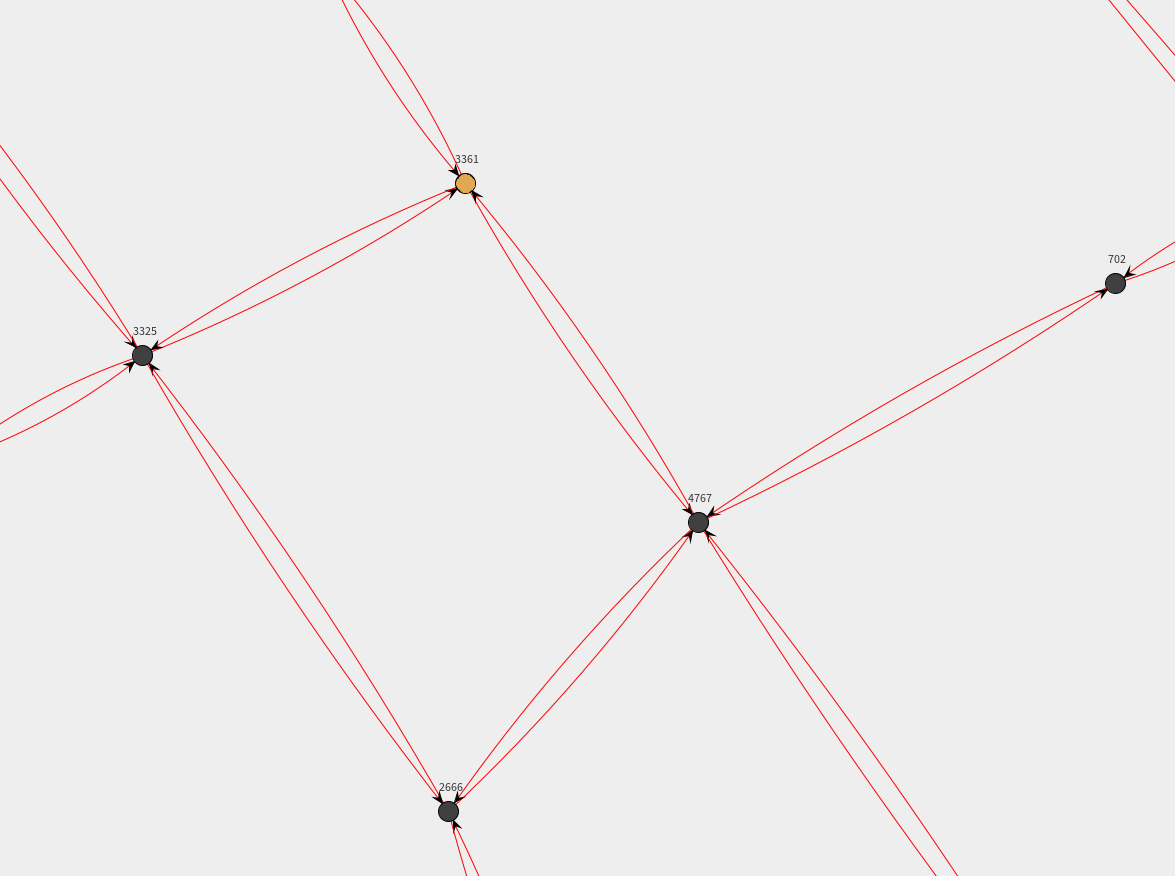
\includegraphics[width=1.0\textwidth]{img/ex_space_dijk.png}
    \end{figure}

  \newpage
  \section{Nearest Neighbour Algorithm}
    Como anteriormente referido, a nossa solução para o problema implementa o
    \textit{Nearest Neighbour Algorithm} como solução para o
    \textit{Travelling Salesman problem} (TSP). O TSP surge aquando procuramos
    o melhor trajeto a seguir de modo a alcançar todos os pontos de encontro
    para cada autocarro (terminando o trajeto na empresa onde os clientes
    trabalham).\\
    A nossa implementação deste algoritmo tem complexidade temporal de
    $O(|M|^2)$, sendo $|M|$ o número de pontos de encontro (determinados
    previamente) para a lista de trabalhadores a deslocar. É de notar que,
    a nossa implementação deste algoritmo depende da distância entre cada par
    de pontos de encontro, garagem e empresa de destino. Para calcular essa
    distância, é usado o algoritmo de Dijkstra\cite{DIJKSTRA} (discutido
    na secção anterior) entre todos esses pares de pontos. A distância
    obtida entre esses pontos é sempre a mais curta possível no grafo.
    Este cálculo tem complexidade temporal de
    $O((|V| + |E|) * \log|V| * |M|^2)$.\\
    \newline
    No que toca a complexidade espacial, esta implementação usa um grafo auxiliar
    representado sob a forma de matriz e um vetor onde guarda a ordem pela qual
    os vértices devem ser visitados no trajeto calculado.
    Isto corresponde a uma complexidade de $O(|M|^2 + |M|)$, em que $|M|$
    representa o número de pontos de encontro a visitar.

  \newpage
  \section{Escolha de Pontos de Encontro}
    A escolha de pontos de encontro é necessária para definir o trajeto para
    cada autocarro. Para tal, implementámos um algoritmo \textit{greedy} que visa
    minimizar o número de pontos de encontro atribuídos, obtendo assim o menor
    itinerário possível.\\
    A estratégia tem complexidade temporal de $O(|V| * |T| + |T| * |V|)$, em que
    $|V|$ corresponde ao número de trabalhadores e $|V|$ o número de vértices do
    grafo. \\
    A primeira parcela refere-se à pesquisa em profundidade por cada trabalhador
    necessária para determinar os seus vértices alcançáveis que, no pior caso
    ($d_{max} = \infty$), implica uma visita por todos os vértices. Contudo, como
    $d_{max}$ assume valores muito pequenos no problema em análise, o número de
    vértices alcançáveis também é reduzido. Por esta razão, a pesquisa, na prática,
    não se aproxima do pior caso.\\
    A segunda parcela corresponde à escolha dos pontos de encontro com maior 
    acessibilidade por todos os trabalhadores. No pior caso é necessário retirar
    todos os trabalhadores $|T|$ de todos os vértices $|V|$ presentes na \textit{priority queue}
    auxiliar. No entanto, é de notar que este caso assume que todos os vértices
    do grafo são pontos de encontro alcançáveis, e que cada um é atingível por
    todos os trabalhadores. É evidente que isto não corresponde à realidade,
    logo o caso real tem melhor complexidade temporal do que o pior caso aparenta.\\
    Em relação à complexidade espacial, esta implementação usa uma \textit{priority queue}
    que, no pior caso, contém todos os vértices no grafo (todos são pontos de encontro alcançáveis).
    Isto leva a uma complexidade de $|V|$.

\chapter{Análise temporal empírica}
  \section{Dijkstra's shortest path algorithm\cite{DIJKSTRA}}
    \begin{figure}[H]
      \centering
      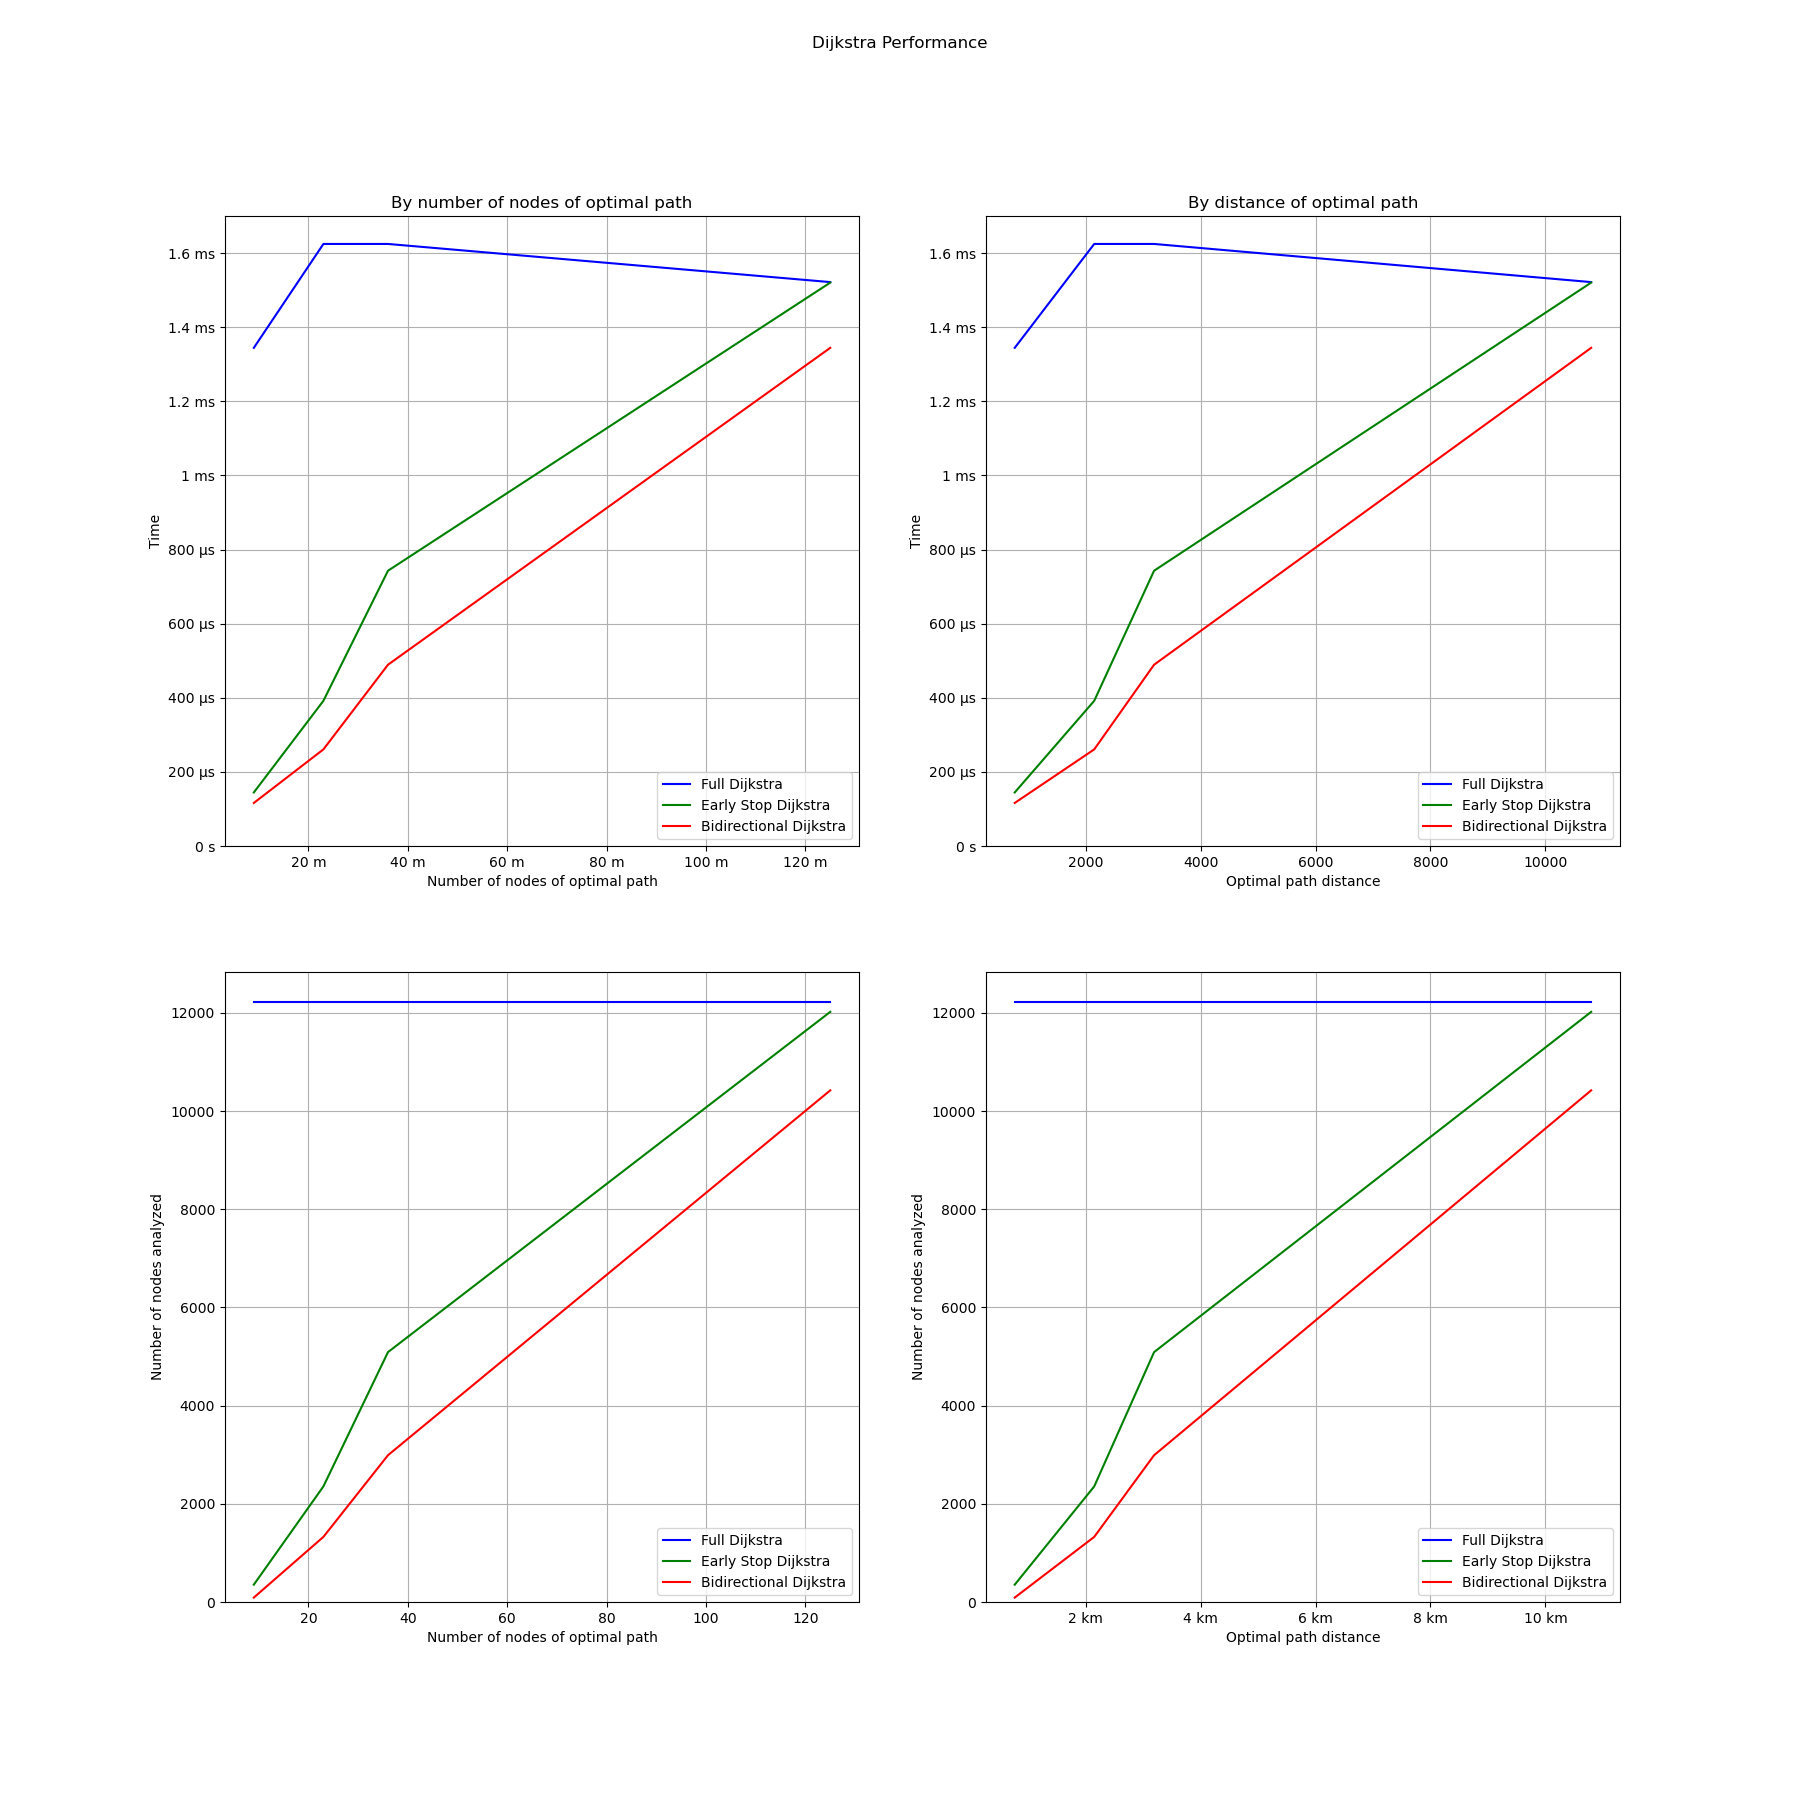
\includegraphics[width=1.0\textwidth]{img/dijkstra_performance.png}
    \end{figure}
    Usamos o algoritmo de Dijkstra para descobrir o caminho mais curto entre dois
    vértices e a distância entre eles (comprimento desse caminho). Esse processo
    é repetido diversas vezes no código pois é necessário saber a distância entre
    cada par de pontos de encontro para que o \textit{Nearest Neighbour Algorithm}
    possa determinar o melhor caminho a seguir.\\
    Com isto em mente, podemos concluir que o desempenho deste algoritmo é decisivo
    para o desempenho total do programa.\\
    Como se pode observar, a implementação deste algoritmo que usávamos inicialmente,
    representada pela linha azul, visitava todos os vértices acessíveis desde do
    vértice dado, o que geralmente conduzia a que praticamente todos os vértices
    do grafo fossem visitados. Isto era extremamente ineficiente, especialmente
    quando considerámos que a distância entre dois pontos de encontro é geralmente
    bastante pequena e que alternámos a origem do percurso a verificar regularmente.
    Para resolver este problema, começamos por implementar uma versão alternativa
    desse algoritmo (representado pela linha verde) que parava as suas iterações
    após encontrar um escolhido ponto de destino. Podemos verificar que esse é
    muito mais rápido que o anterior, especialmente quando o número de vértices
    (similar a distância) entre os dois pontos, origem e destino, é baixo.\\
    Após algum tempo, fizemos uma outra melhoria a este algoritmo (representada
    pela linha vermelha nos gráficos) que envolve uma pesquisa bidirecional pelo
    algoritmo de Dijkstra, ou seja, o algoritmo corre em simultâneo desde a origem
    para o destino e do destino para a origem, encontrando-se a meio desse percurso
    se existir caminho entre os dois pontos. É de notar que esta estratégia é mais
    rápida, mas implica que um pós-processamento dos resultados e que o grafo
    utilizado seja fortemente conexo. Este último tópico irá ser discutido mais
    tarde no relatório.

  \section{Nearest Neighbour Algorithm\cite{PSEUDONNA}}
    \begin{figure}[H]
      \centering
      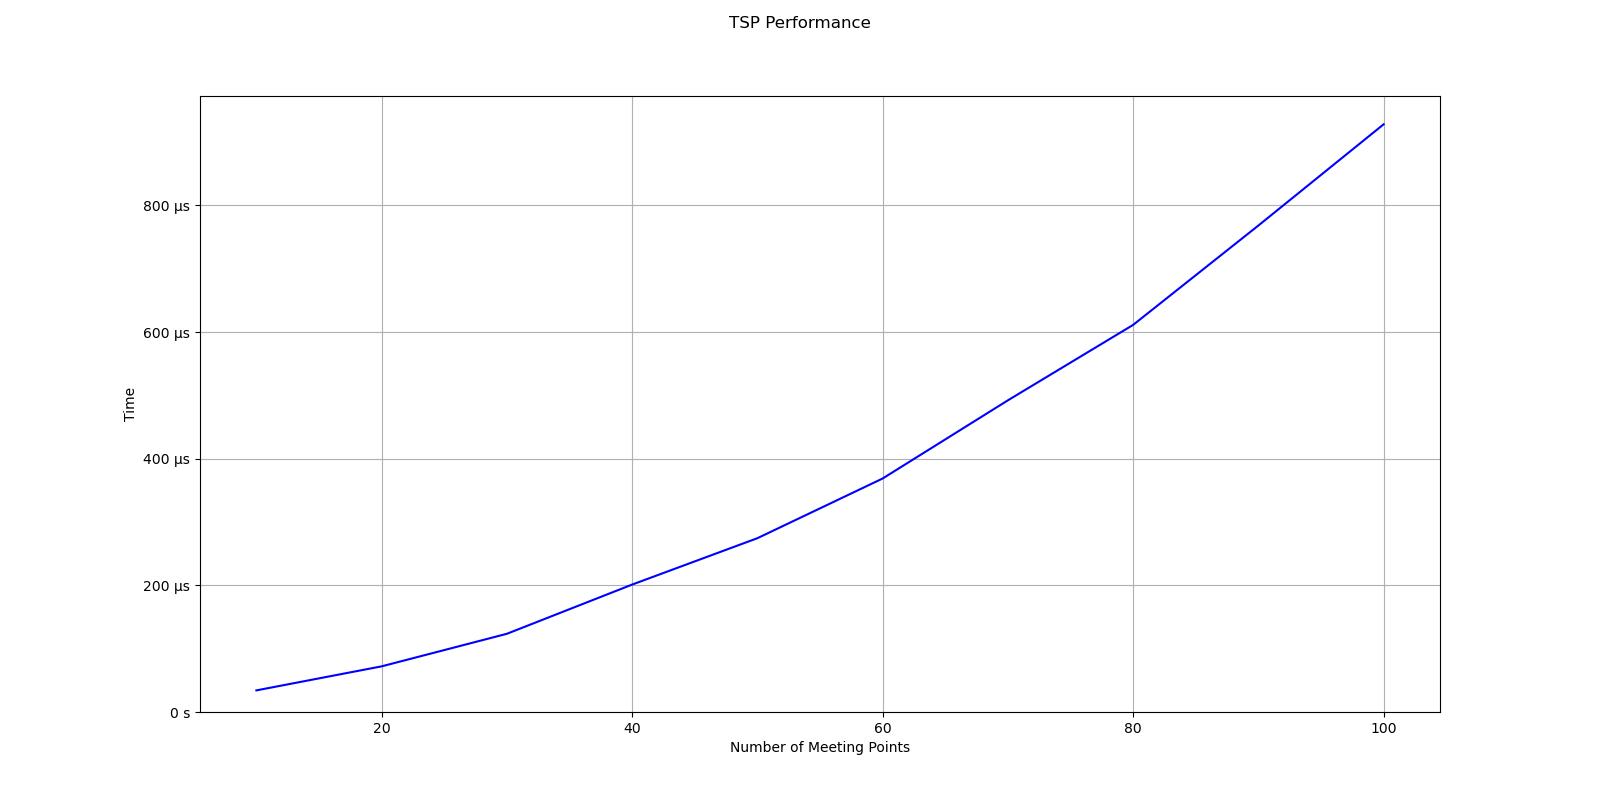
\includegraphics[width=1.0\textwidth]{img/tsp_performance.png}
    \end{figure}
    Como já foi referido anteriormente, a escolha do caminho ótimo que passa por
    todos os pontos de encontro, começando na garagem e terminando na empresa
    cliente de destino é uma versão alternativa do TSP\cite{TSP}.\\
    Foi implementado o \textit{Nearest Neighbour Algorithm}\cite{PSEUDONNA} para
    dar uma solução aproximada, embora por vezes grosseiramente, a esse problema
    dada a sua simplicidade e eficiência de execução (complexidade polinomial).\\
    Este algoritmo é executado uma vez para cada empresa cliente que esteja a
    ser tratada, o que é perfeitamente aceitável dada a sua eficiência de execução,
    mesmo para casos com elevada quantidade de pontos de encontro
    (100 pontos de encontro $\approx 8.5ms$).

  \section{Escolha de Pontos de Encontro}
    \begin{figure}[H]
      \centering
      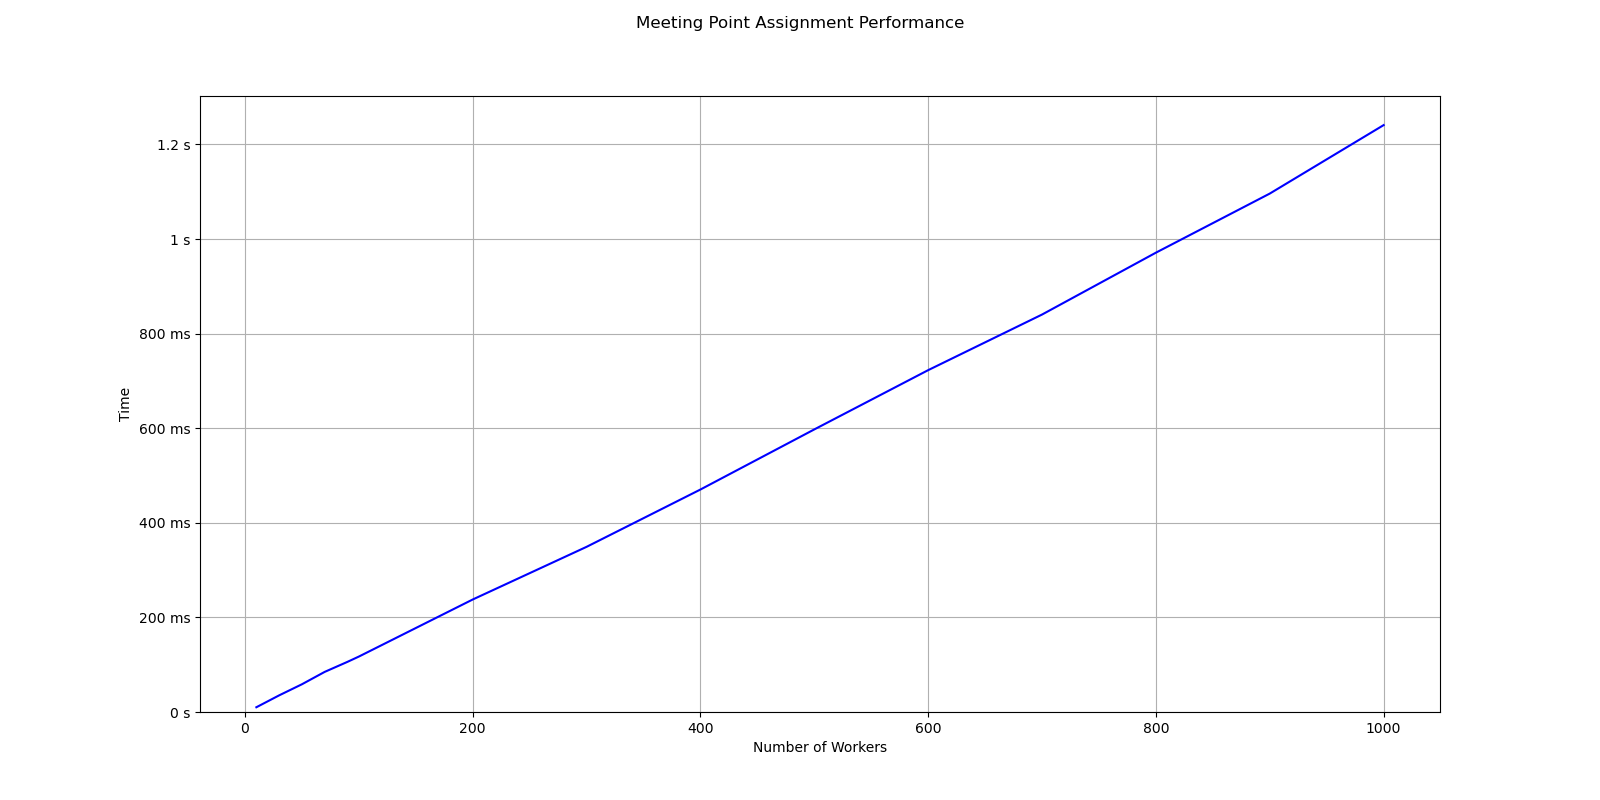
\includegraphics[width=1.0\textwidth]{img/meetAssign_performance.png}
    \end{figure}
    O desempenho deste algoritmo varia com os valores de $d_{max}$, com número de
    paragens de autocarro no grafo e com o número de trabalhadores a processar.\\
    De modo a simplificar a análise, estes testes foram feitos no mesmo grafo e
    variando apenas o número de trabalhadores a processar. Isto também é a análise
    mais próxima dos casos de uso real do programa, pois numa cidade o número de
    paragens de autocarro permanece constante e a $d_{max}$ é constante ao longo
    de cada execução do programa.\\
    Os valores no gráfico foram obtidos usando $d_{max} = 1000 (1km)$ e 1100 paragens
    de autocarro escolhidas aleatoriamente antes da primeira execução do código.

\chapter{Grafos utilizados e sua conectividade}
  Durante a fase inicial de desenvolvimento, foram utilizados os \textit{Grid graphs}
  e o mapa do porto disponibilizados na página do \textit{moodle} da unidade curricular.
  Após algum tempo, não estávamos satisfeitos com esses grafos, pelo que criámos o
  nosso próprio grafo, representativo da cidade do Porto (Portugal), para uso
  demonstrativo no projeto.\\
  Para esse efeito, fizemos uma \textit{query} da base de dados do \textit{Open Street
  Map} usando a \textit{Overpass API} e, posteriormente, usamos alguns
  \textit{Python Scripts} para trabalhar essa informação, simplificando-a e adaptando-a
  à nossa situação. Estes \textit{scripts} estão disponíveis no diretório \textbf{import}
  do projeto.\\
  O grafo que utilizamos não é fortemente conexo, então foi implementada uma rotina de
  extração do sub-grafo fortemente conexo do grafo importado, que contém a garagem. Isto
  permite evitar problemas de execução difíceis de detetar \textit{a priori}, como por
  exemplo, as coordenadas de moradia de um trabalhador colocarem-no num vértice inacessível
  a partir da garagem.\\
  O nosso programa foi maioritariamente testado nos nossos grafos, mas, como base nos
  nossos testes, caso o formato da informação nos grafos disponibilizados pela
  unidade curricular seja convertido para aquele usado no nosso programa, irão
  funcionar também.

\chapter{Conclusão}
  Acreditamos ter atingido todos os nossos objetivos planeados para este projeto
  com a adição de algumas funcionalidades extra.\\
  No entanto, gostávamos de ter implementado um algoritmo melhor para obter
  uma solução aproximada do TSP\cite{TSP}, pois o
  \textit{Nearest Neighbour Algorithm}\cite{NNA} tem várias falhas e é aquele
  que faz da nossa solução uma aproximação ao resultado ótimo. Mesmo com isto
  em mente, acreditamos ter obtido soluções bastante aceitáveis ao problema
  proposto.\\
  O grafo que preparamos está completo e representa bem a cidade do Porto o que
  torna os resultados mais interessantes de observar. Por outro lado, gostávamos
  de ter trabalhado um pouco mais os menus/interface com o utilizador e incluir
  todas as funções de CRUD no código para as informações importadas de ficheiros.\\
  Durante o desenvolvimento do projeto apercebemo-nos que o 3º problema proposto 
  (Determinação de rotas para vários autocarros com um só destino) é
  uma instância do \textit{Vehicle Routing Problem (VRP)\cite{VRP}}. Logo de seguida, concluímos
  que o 4º problema (Determinação de rotas para vários autocarros para várias empresas)
  trata-se do \textit{Routing Problem with Pickup and Delivery (VRPPD)\cite{VRP}}. Determinar a
  solução otíma tanto para o VRP como para o VRPPD é um problema NP-Hard\cite{VRP}.
  No geral, as soluções obtidas para estes problemas poderão ser mais custosas do que as soluções ótimas,
  mas, por outro lado, são calculadas de forma muito mais eficiente.
  O fator que conduz a esta situação é o facto de ser assumido que um autocarro deve apenas levar
  trabalhadores de uma só empresa.\\
  O trabalho foi distribuído de forma igual por todos os elementos do grupo.

\newpage
\chapter{Créditos}
Agradecemos ao \href{https://www.openstreetmap.org}{\textit{Open Street Map}}
e aos seus contribuidores, à
\href{https://wiki.openstreetmap.org/wiki/Overpass_API}{\textit{Overpass API}}
e ao \href{https://overpass-turbo.eu/}{\textit{Overpass Turbo}} que
possibilitaram a obtenção e uso do mapa que trabalhamos no nosso projeto.\\
\newline
Também queremos agradecer ao utilizador do
\href{https://github.com/rovaniemi}{\textit{GitHub} rovaniemi} pela
disponibilização da aplicação
\href{https://github.com/rovaniemi/osm-graph-parser}{\textit{OSM Graph Parser}}
que fez a tradução da informação no mapa para o formato JSON.

\newpage
\bibliography{biblio}
\bibliographystyle{ieeetr}

\end{document}
